%!TEX root = ../main.tex
%-------------------------------------------------------------------------------
%                     BAB III
%               			PEMBAHASAN
%-------------------------------------------------------------------------------


\chapter{METODOLOGI PENELITIAN}

\section{Tahapan Penelitian}

\begin{figure}[H]
  \centering{}
	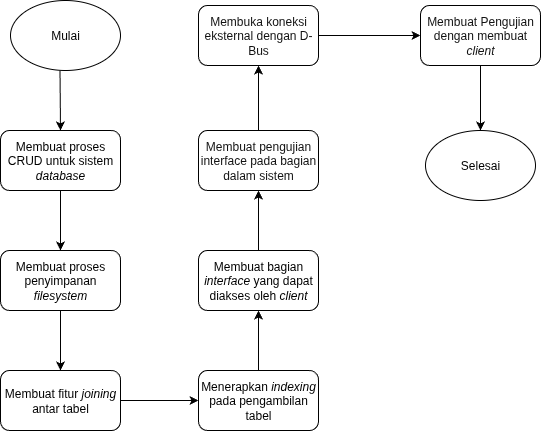
\includegraphics[width=0.9\textwidth]{gambar/bab4/Tahapan-Penelitian-Baru}
  \caption{Alur tahapan penelitian pembuatan \emph{database engine}}
\end{figure}

Penelitian dimulai dengan mencoba menerapkan fungsional dasar (CRUD) pada \emph{database} yaitu proses pengambilan,
penambahan, pengubahan dan penghapusan data. Pengembangan fungsi-fungsi dasar akan melibatkan berbagai macam struktur
data. Langkah pertama dari belum bisa memiliki data yang persisten karena data yang diolah pada langkah ini belum 
terhubung ke \emph{filesystem}.

Langkah berikutnya yaitu penerapan penyimpanan secara persisten di \emph{filesystem}. Meneruskan proses-proses data yang telah
masuk di langkah pertama dan membuat data tersimpan pada \emph{filesystem}. Setelah penyimpanan berhasil dibuat, dilanjutkan dengan proses pembuatan
fitur \emph{joining} antar tabel. Proses \emph{joining} ini akan melakukan penggabungan data dari 2 tabel yang terpisah. Setelah berhasil melakukan \emph{join} tabel, pengembangan fitur \emph{indexing}
akan dilakukan. Fitur \emph{indexing} akan berjalan ketika hendak melakukan pengambilan data pada saat melakukan \emph{join} tabel. Dengan memanfaatkan fitur \emph{indexing},
penerapan fitur \emph{joining} tabel akan dilakukan agar proses penggabungan tabel menjadi lebih cepat.

Setelah fungsi-fungsi berhasil dibuat, maka diperlukan sebuah \emph{interface} untuk memisahkan fungsi mana saja yang dapat diakses oleh pengguna dan fungsi mana
yang hanya bisa diakses oleh sistem. Fungsi pada \emph{Interface} ini yang nanti akan dibuka dan dapat diakses oleh pengguna. Lalu untuk memastikan
fungsi-fungsi yang telah dibuat berjalan dengan baik, dibuatlah \emph{interface} untuk melakukan pengujian secara internal. Interface pengujian internal dibuat berdasarkan fungsi
pada interface yang telah dibuat sebelumnya (\emph{Interface} untuk fungsi pengguna). Maksud dari internal disini adalah proses pengujian dilakukan dengan menggunakan bahasa 
pemrograman yang sama yaitu rust, dan fungsi di panggil secara langsung tanpa melalui koneksi external seperti D-bus.  

Setelah pembuatan \emph{interface} pengujian internal, pembuatan interface koneksi D-Bus dibuat, disusul dengan pembuatan pengujian eksternal menggunakan bahasa pemrograman
lain untuk memastikan koneksi D-Bus berjalan dengan baik. Berikut adalah linimasa dari tahapan penelitian. Linimasa ini hanyalah perkiraan awal dan estimasi dari waktu 
pengembangan \emph{database engine}.


\begin{table}[H]
  \centering{}
  \begin{tabular}{|m{0.8cm}|m{7cm}|m{5cm}|}
      \hline
      \textbf{No.} & \textbf{Tahapan} &  \textbf{Estimasi Waktu} \\
      \hline
      1. & Membuat proses \emph{CRUD} untuk \emph{interface database} & 3 pekan \\
      \hline
      2. & Membuat Proses Penyimpanan \emph{Filesystem} & 1 bulan \\
      \hline
      3. & Membuat fitur \emph{joining} tabel & 2 pekan \\
      \hline
      4. & Menerapkan \emph{indexing} & 2 pekan \\
      \hline
      5. & Membuat \emph{interface} yang dapat diakses pengguna & 1 Pekan \\
      \hline
      6. & Membuat pengujian untuk \emph{interface} pada bagian dalam sistem & 1 Pekan \\
      \hline
      7. & Membuka koneksi external dengan D-Bus & 1 Pekan \\
      \hline
      8. & Membuat pengujian eksternal dengan membuat \emph{client} & 1 Pekan \\
      \hline
  \end{tabular}
  \caption{Tabel linimasa perkiraan awal dan estimasi pengerjaan}
\end{table}

\section{Penerapan Kebutuhan Fitur}
Berdasarkan subbab 2.2, \emph{database} memiliki beberapa fitur umum yang dapat berfungsi untuk mengolah data. 
Untuk proses pengembangan \emph{database engine}, fitur-fitur umum yang ada pada \emph{database} 
akan dikembangkan. Beberapa fitur tersebut di antaranya adalah:
\begin{enumerate}
	\item Kemampuan untuk Membaca data (\emph{Read}) \\
	Fitur ini berguna untuk melakukan pengambilan data yang berasal dari sebuah \emph{file} yang telah disimpan pada \emph{filesystem}.

	\item Kemampuan untuk melakukan proses penyimpanan dan mengolah data secara persisten (\emph{Create, Update dan Delete}) \\
	Proses penyimpanan dan hasil pengolahan data akan disimpan secara persisten pada \emph{filesystem} dengan menggunakan format
  tersendiri. 


	\item Penggunaan \emph{Index} \\
	Penerapan \emph{indexing} sederhana akan diterapkan terhadap data yang ada dalam \emph{database}

	\item Penggabungan 2 tabel (\emph{Join}) \\
	Kapabilitas untuk melakukan \emph{joining} 2 tabel terhadap data yang telah disimpan

	\item Koneksi servis \emph{Client} via \emph{D-Bus} \\	
  Fitur untuk menerima proses permintaan dari \emph{client} untuk menjalankan fungsi-fungsi yang ada dalam \emph{database}.
			
\end{enumerate}

\section{Arsitektur Struktur Data}

Sistem \emph{database} terdistribusi dilakukan dengan melakukan pemecahan penyimpanan 
\emph{database} pada mesin yang berbeda. Setiap mesin \emph{database} yang terpisah dapat 
berkomunikasi satu sama lain namun tidak secara langsung. Dibutuhkan 2 mesin 
tambahan yang berguna untuk menghubungkan \emph{database} terpisah tersebut. Berikut 
adalah ilustrasi dari arsitektur yang akan diterapkan:
\begin{figure}[H]
  \centering{}
  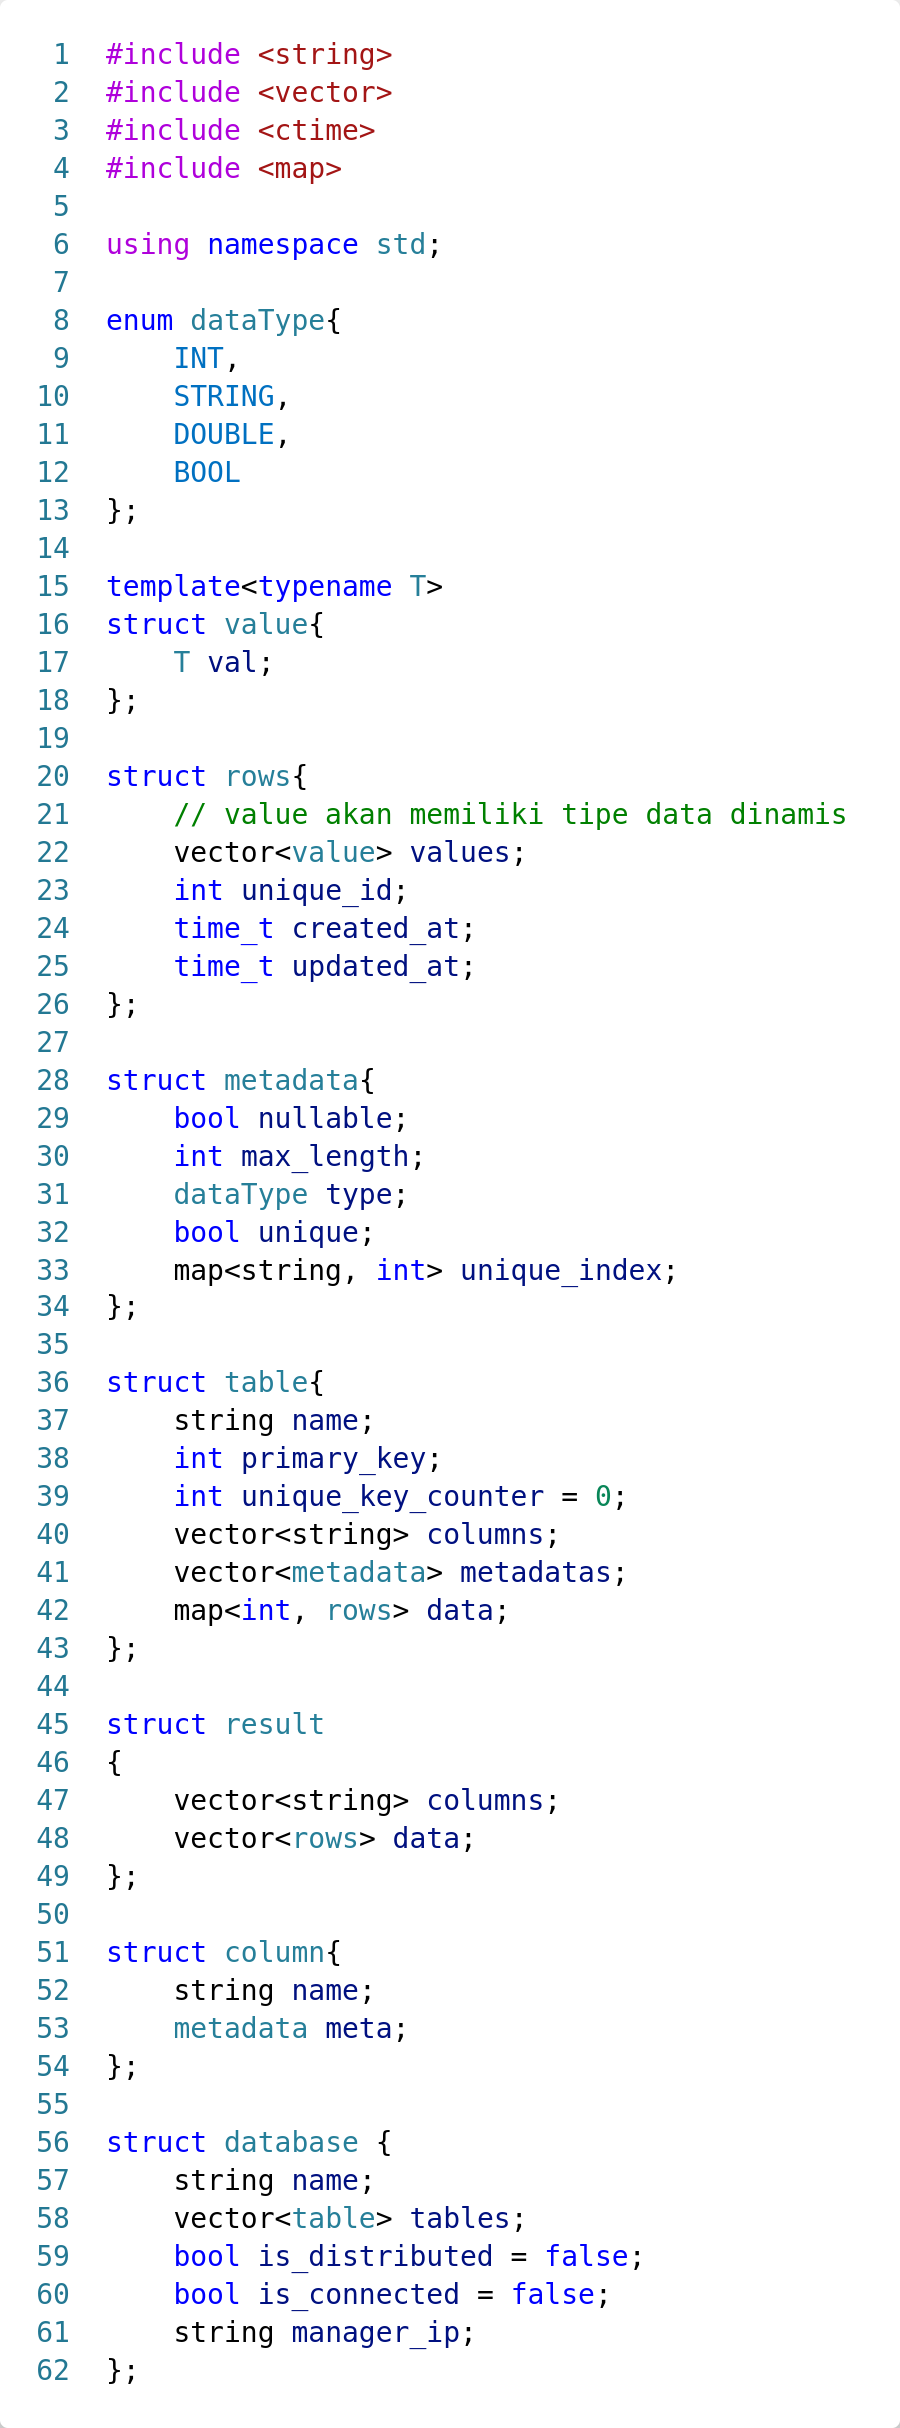
\includegraphics[width=0.5\textwidth]{gambar/bab3/structure_struct_database}
  \caption{Contoh penerapan \emph{struct} \emph{database} pada bahasa C++}
\end{figure}

Terdapat beberapa atribut dalam \emph{class} tabel di antaranya adalah name yang akan 
menampung nama dari tabel, primary\_key yang akan menampung kolom mana yang akan 
menjadi primary key, column yang merupakan array \emph{string} berisi urutan nama kolom 
pada tabel, lalu metadata merupakan array dari \emph{class} metadata yang berisi metadata 
berkaitan dengan kolom yang ada sesuai dengan urutan dan terakhir terdapat atribut 
data. Attribut data ini akan berisi \emph{hashmap} dengan key unique id dengan value 
\emph{class} rows. \emph{Value} unique id berasal dari atribut unique\_key\_counter yang memiliki 
default \emph{value} 0 dan akan terus bertambah ketika terdapat \emph{row} baru yang masuk ke dalam 
hashmap.

Pada penerapan \emph{class} rows, terdapat atribut unique\_id, created\_at dan updated\_at. 
Untuk atribut unique\_id akan berisi sebuah integer yang berasal dari key penyimpanan 
rows di \emph{class} tabel. Atribut created\_at dan updated\_at akan memiliki \emph{value} epoch 
timestamp yang berasal dari waktu data dibuat dan waktu data di diubah. Atribut 
created\_at juga memiliki peran pada saat melakukan penerapan sinkronisasi. Lalu pada 
bagian row memiliki array dari \emph{class values}. \emph{Class} ini memiliki \emph{interface Get Value} 
yang berguna untuk mengembalikan \emph{value} generik yang ada dalam \emph{class values}. Penerapan 
seperti ini dilakukan agar \emph{value} yang disimpan dapat dinamis. 

\emph{Class} column yang dibuat pada gambar, berguna ketika menampilkan semua column beserta 
metadata nya. Terdapat \emph{class} metadata yang akan menyimpan informasi terkait column 
yang ada seperti tipe kolom, \emph{nullable} dan lainnya. Di dalam \emph{class} metadata terdapat 
sebuah hashamp yang akan digunakan sebagai \emph{index}. \emph{Index} ini berfungsi untuk mempercepat 
pencarian terhadap sebuah \emph{value} sehingga akan digunakan ketika column memiliki tipe 
unik dan ketika hendak melakukan sinkronisasi data ketika menerapkan sistem 
terdistribusi. \emph{Hashmap} akan memiliki \emph{key value pair} dengan \emph{key} yang berisi \emph{value} dari 
kolom yang di \emph{index} sementara untuk \emph{value} dari hashmapnya adalah unique id yang 
berasal dari \emph{key} penyimpanan rows pada \emph{class} table. Enum dataType yang ada pada 
metadata berguna untuk membatasi tipe data yang akan dipakai pada column \emph{database}.

Terakhir terdapat \emph{database} \emph{class} atau \emph{struct} yang merupakan \emph{parent} dari semua \emph{class}. 
\emph{Database class} mempunyai atribut table yang merupakan array dari \emph{table} \emph{Class}. 
\emph{Database class} juga mempunyai atribut name yang dibutuhkan ketika saat 
mendeklarasikan \emph{class} tersebut. Dalam \emph{class} yang dibuat akan mengimplementasikan 
\emph{interface} nya masing-masing. \emph{Interface} ini akan berisi metode atau \emph{function} yang 
berguna untuk menjalankan operasi dalam \emph{database}.

Berikut ini adalah isi metode atau \emph{function} yang ada dalam \emph{interface \emph{class} database}:
\begin{enumerate}
	\item \emph{Get Table} \\
	Berguna untuk mengambil \emph{instance} \emph{class table} yang berada dalam \emph{class database}. 
  \emph{Method} ini menerima 1 \emph{parameter} berupa \emph{string} yang isinya adalah nama table dari 
  list \emph{instance} yang ada dalam \emph{database}. Hasil dari \emph{return} \emph{method} ini adalah \emph{instance} 
  table yang mempunyai nama yang sama dengan \emph{value} yang ada di \emph{parameter}.


	\item \emph{Create Table} \\
  \emph{Method} ini berguna untuk menambahkan \emph{class table} baru ke dalam \emph{database}. Menerima 1 
  \emph{parameter} berupa \emph{class table} yang nantinya \emph{instance} tersebut akan dimasukkan ke 
  dalam list \emph{class table} pada \emph{database}. Hasil dari \emph{return method} ini adalah \emph{class 
  table} yang sudah berhasil dibuat. 


	\item \emph{Delete Table} \\
  \emph{Method} ini berguna untuk menghapus tabel yang ada pada \emph{class database}. Menerima 1 
  \emph{parameter} berupa \emph{string} yang isinya adalah nama \emph{table} yang ingin dihapus dalam 
  \emph{database}.

  
	\item \emph{Get Database Name} \\
  \emph{Method} ini berfungsi untuk mengambil nama dari \emph{database}, tidak akan menerima 
  \emph{parameter} apapun dan akan mengembalikan return sebuah \emph{string} nama dari \emph{database}.


	\item \emph{Update Database Name} \\
  \emph{Method} ini berfungsi untuk Mengganti nama dari \emph{database}, akan menerima 1 \emph{parameter} 
  berupa \emph{string} yang isinya adalah nama \emph{database} terbaru yang ingin diubah.


	\item \emph{Read File} \\
  \emph{Method} ini berfungsi untuk membaca data yang sudah disimpan secara persisten pada 
  \emph{virtual file system}. Attribute list \emph{table} nantinya akan diisi melalui \emph{method Read 
  File} ini.


	\item \emph{Write File} \\
  Berfungsi untuk menyimpan data secara persisten dan menuliskannya ke \emph{file} yang 
  telah ditentukan.


	\item \emph{Create File} \\
  Berfungsi untuk membuat \emph{space} baru ketika \emph{database} ingin dibuat. \emph{Method} ini 
  dijalankan hanya jika belum ada \emph{space} untuk \emph{database}.


	\item \emph{Set Distributed} \\
  Berfungsi untuk memberikan informasi kepada \emph{database} untuk berjalan secara 
  terdistribusi. \emph{Method} ini menerima 2 \emph{parameter}, \emph{parameter} pertama adalah boolean 
  untuk menentukan apakah berjalan terdistribusi atau tidak. Lalu untuk \emph{parameter} 
  kedua berisi IP dari manajer untuk menerapkan sistem terdistribusi. 
  
\end{enumerate}

Dalam \emph{database} nantinya akan terdapat list \emph{class} table. \emph{Class} table juga akan memiliki \emph{method} yang berguna untuk melakukan pengolahan data. Berikut ini adalah\emph{interface} yang ada pada \emph{class} table:

\begin{enumerate}
	\item \emph{Get Data} \\
	Berguna untuk mengambil data yang tersedia dalam \emph{class} table. \emph{Method} ini akan 
  memiliki dua \emph{parameter}, \emph{parameter} \emph{hashmap} yang di dalamnya terdapat key dan value 
  yang sama dengan kolom pada table. Hal ini berfungsi untuk mencari value yang 
  tersedia pada data yang ada dalam \emph{class} table. \emph{Parameter} kedua akan berperan 
  sebagai konfigurasi pada query seperti mengatur urutan atau melakukan limitasi.

  Dalam \emph{method} ini terdapat proses pengambilan data yang diambil dari storage 
  persisten. Hasil akhir dari \emph{method} ini berupa \emph{class} result yang berisi atribut 
  column dan row tanpa metadata dengan ketentuan yang diberikan pada \emph{parameter}.


	\item \emph{Show Data} \\
	Method Show Data berguna untuk mengambil satu buah data yang sesuai dengan id 
  yang diberikan. \emph{Method} ini akan mengembalikan \emph{class} result.


	\item \emph{Create Data} \\
  \emph{Method} yang berguna untuk membuat data / \emph{row} baru pada \emph{class table}. \emph{Method} 
  ini menerima 1 \emph{parameter}, yaitu \emph{hashmap} yang berisi \emph{key} dan \emph{value} yang sesuai 
  dengan kolom yang ada pada table yang dituju. Untuk \emph{hashmap} yang disediakan 
  harus menyesuaikan dengan metadata yang dibuat pada \emph{class table}. Jika terdapat 
  kolom yang tidak \emph{nullable}, maka \emph{value} dari kolom tersebut harus ada pada 
  \emph{hashmap} yang disediakan. Hasil Return dari \emph{method} ini adalah \emph{class result} yang 
  sudah berisi data-data yang diminta untuk dibuat.  

  \emph{Method} ini akan mengirimkan \emph{event} ke manajer sebelum melakukan penyimpanan 
  jika \emph{database} berjalan secara terdistribusi. Lalu juga akan melakukan perubahan 
  pada unique\_index pada \emph{class} metadata jika kolom mempunyai \emph{value} yang unik.

  
	\item \emph{Update Data} \\
  \emph{Method} \emph{update} ini berguna untuk mengubah sebuah data yang ada di dalam \emph{class 
  table} dengan ketentuan yang telah diberikan. \emph{Method} ini akan menerima 2 
  \emph{parameter}, \emph{parameter} pertamanya adalah \emph{hashmap} yang nantinya digunakan untuk 
  mencari data yang sesuai. Lalu untuk \emph{parameter} kedua juga akan berisi 
  \emph{hashmap} yang terdiri dari \emph{key} dan \emph{value} yang ingin diubah. Hasil Return dari 
  \emph{method} ini adalah \emph{class} result yang sudah berisi data terbaru yang telah 
  diubah. Jika terdapat column yang memiliki \emph{index}, maka \emph{value} \emph{index} tersebut 
  juga akan di \emph{update}. Termasuk jika menerapkan \emph{database} terdistribusi, maka akan 
  mengirimkan \emph{event} ke manajer untuk memastikan data yang di-\emph{update} tidak 
  duplikasi dengan data di mesin lain.

  
	\item \emph{Delete Data} \\
  Berguna untuk menghapus data yang ada dalam \emph{class table}. \emph{Method} ini menerima 1 
  \emph{parameter}, \emph{parameter} pertamanya adalah \emph{hashmap} yang akan menentukan data mana 
  yang akan di hapus. Isi dari \emph{hashmap} harus sesuai dengan kolom yang tersedia 
  pada \emph{class table}. \emph{Method} ini akan mengembalikan status apakah dia berhasil 
  menghapus data atau tidak. Jika terdapat kolom yang mempunyai \emph{index}, maka 
  \emph{index} tersebut juga akan dihapus.

  
	\item \emph{Get Column} \\
  \emph{Method} ini berguna untuk mengambil \emph{list column} yang ada pada \emph{class table} beserta 
  dengan metadata nya. \emph{Method} ini tidak menerima \emph{parameter} apapun dan akan 
  mengembalikan sebuah array dari \emph{class column}.
 
  
	\item \emph{Create Column} \\
  \emph{Method} ini berguna untuk menambahkan \emph{column} baru pada \emph{class table}. Terdapat 1 
  \emph{parameter} dalam \emph{method} ini yaitu \emph{instance} \emph{column} yang nantinya akan dimasukkan 
  ke dalam \emph{list columns} yang tersedia pada table. Lalu untuk penambahan \emph{column} 
  ini, nantinya pada bagian \emph{row} data juga akan ikut bertambah data kosong atau 
  default \emph{value} dari \emph{column} yang baru saja ditambahkan.
 
  
	\item \emph{Update Column} \\
  Berguna untuk mengganti nama \emph{column}. \emph{Method} ini akan menerima 1 \emph{parameter} 
  berupa \emph{string} yang isinya merupakan nama baru dari \emph{column} yang ingin diubah. 
  Hasil \emph{return} dari \emph{method} ini adalah instance \emph{column} yang datanya berhasil diubah.
  
 
	\item \emph{Delete Column} \\
  Berfungsi untuk menghapus \emph{column} beserta data dari \emph{column} tersebut. \emph{Method} 
  ini hanya menerima 1 \emph{parameter} saja yaitu nama dari \emph{column} yang ingin kita 
  hapus sehingga \emph{parameter} ini akan mempunyai tipe data \emph{string}. Hasil \emph{return} 
  dari \emph{method} ini adalah status keberhasilan penghapusan \emph{column}.  
 
\end{enumerate}


\section{Alur Penyimpanan Data kepada \emph{Filesystem}}

Data akan disimpan secara persisten ke dalam \emph{filesystem} dalam bentuk \emph{bytes}, sehingga terdapat 
beberapa tahapan untuk melakukan penyimpanan ke \emph{filesystem}. \emph{Client} akan melakukan pengolahan 
data melalui \emph{interface database} yang disediakan. Terdapat proses pengambilan data dan proses penyimpanan 
data. Kedua proses ini mempunyai alur yang mirip namun ada sedikit perbedaan. 

Untuk proses pengambilan data, \emph{database engine} akan terlebih dahulu melakukan pengecekan, apakah 
\emph{database} atau tabel yang dituju tersedia atau tidak. Jika tidak, maka \emph{database} atau tabel
belum dibuat atau tidak ada sehingga diperlukan pembuatan terlebih dahulu. Namun, Jika \emph{database} atau tabel 
tersedia maka langkah berikutnya adalah melakukan pengubahan data dari \emph{bytes} ke tipe datanya.
Tipe data ini akan tersedia di dalam \emph{bytes} yang disimpan pada \emph{filesystem}.  Setelah berhasil melakukan pengubahan,
maka data tersebut akan disimpan secara sementara pada atribut yang ada di dalam struktu data \emph{database}.
Berikut adalah alur pengambilan data dalam bentuk diagram:

\begin{figure}[H]
  \centering{}
	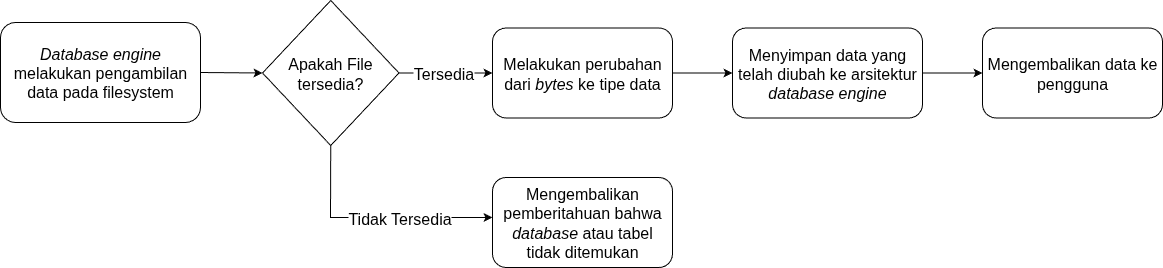
\includegraphics[width=0.9\textwidth]{gambar/bab3/proses-pengambilan-data-filesystem}
  \caption{Proses pengambilan data dari \emph{filesystem}}
\end{figure}

Pada bagian proses pembuatan dan penyimpanan data, memiliki alur yang sama dengan pengambilan data, namun terdapat proses tambahan,
yaitu data harus dikembalikan dalam bentuk \emph{bytes} dan disimpan di dalam \emph{filesystem}. Proses ini dimulai dari \emph{client} 
yang akan menjalankan proses \emph{insert} pada \emph{interface database}. \emph{Database engine} akan melakukan hal yang sama yaitu
pengambilan data, namun jika tabel yang dituju tidak tersedia maka akan mengembalikan sebuah pemberitahuan bahwa tabel tak bersedia. 
Setelah data berhasil diambil dari \emph{filesystem} dan disimpan ke dalam atribut, maka proses perubahan dari data ke \emph{bytes} akan dilakukan.
Data yang telah berubah menjadi \emph{bytes} akan disimpan ke dalam \emph{filesystem}. Berikut adalah alur dari proses penyimpanan jika data 
dalam atribut \emph{database} tersedia:


\begin{figure}[H]
  \centering{}
	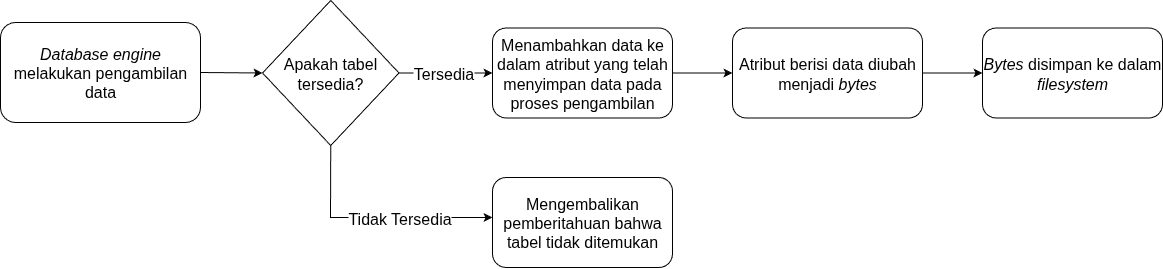
\includegraphics[width=0.9\textwidth]{gambar/bab3/proses-penyimpanan-data-filesystem}
  \caption{Proses penyimpanan data ke \emph{filesystem}}
\end{figure}

\section{\emph{Index} Sederhana dengan \emph{Map}}
Untuk proses \emph{indexing} pada \emph{database engine}, akan memanfaatkan struktur data bernama \emph{Map}. Struktur data \emph{map} yang digunakan mengikuti \emph{library} 
standar pada bahasa pemrograman yang akan digunakan. Dengan menggunakan \emph{map} yang ada dalam bahasa pemrograman, maka tidak perlu membuat struktur data khusus
untuk menerapkan \emph{index} pada \emph{database}. Karena menggunakan \emph{library} standar, struktur data ini juga akan memiliki \emph{function} yang dapat digunakan untuk mempermudah
proses pengembangan. Selain memiliki \emph{function-function} yang dapat digunakan, \emph{Map} yang tersedia pada \emph{library} standar bahasa pemrograman umumnya dapat 
menyimpan berbagai jenis tipe data. Penerapan \emph{Map} di arsitektur \emph{database engine} ini kemungkinan akan diterapkan dengan struktur data yang lain seperti \emph{array}.

\section{\emph{Join} Antar Tabel}
Sesuai dengan pernyataan pada batasan masalah, fitur \emph{join} yang ada pada \emph{database engine} awal ini adalah melakukan \emph{join} antar 2 tabel saja.
Prinsip \emph{join} yang digunakan sama seperti \emph{join} yang dilakukan pada \emph{database relational} lainnya, yaitu dengan menggunakan \emph{foreign key}.
Untuk menghubungkan kedua tabel dalam satu \emph{database}, maka terdapat satu kolom (biasanya berupa ID) dalam sebuah tabel yang nilai kolom dari tabel tersebut
merujuk ke tabel lain. Jika terdapat baris dengan nilai sama pada kolom yang telah ditentukan antar tabel, maka baris tersebut akan dianggap menjadi 1 baris.
Perlu diketahui bahwa fitur \emph{join} ini masih bersifat mirip seperti \emph{LEFT JOIN} yang ada di \emph{relational database} dan baru bisa dilakukan antar 2 tabel.


\section{Komunikasi Interface \emph{Database} dengan D-Bus}

Komunikasi dengan D-Bus akan menggunakan \emph{library} D-Bus yang tersedia pada bahasa pemrograman
yang digunakan. Pembuatan koneksi ini menggunakan bahasa pemrograman yang sama dengan bahasa pemrograman yang digunakan
dalam pengembangan \emph{database engine}. Namun, meski dibuat dengan satu bahasa pemrograman, koneksi D-Bus tetap bersifat universal (Dapat digunakan pada sistem lain). 
Sehingga jika \emph{client} menggunakan bahasa pemrograman lain, koneksi D-Bus tetap bisa terhubung satu sama lain. 

Koneksi pada D-bus ini akan dihubungkan melalui path yang nanti akan ditentukan
sebagai path dari jalur koneksi \emph{database engine}. \emph{Client} harus mendefinisikan \emph{path} yang sama dengan 
\emph{database engine} agar bisa terhubung. Dengan koneksi ini, pihak \emph{client} dapat menjalankan fungsi-fungsi 
\emph{database engine} berdasarkan\emph{interface} yang telah dibuka. \emph{Interface} yang dibuka hanyalah
interface yang dapat berguna bagi \emph{client} dan bukan \emph{interface} yang bersifat \emph{low-level}.



\section{Alat dan Bahan}

Untuk melaksanakan penelitian terdapat alat dan bahan yang dibutuhkan, di antaranya 
adalah:
\begin{itemize}
	\item {
    Laptop yang mempunyai spesifikasi untuk menjalankan bahasa pemrograman \emph{rust} dan \emph{python}. Versi bahasa
    pemrograman yang digunakan saat pengembangan adalah rust versi 1.84.1 dan python versi 3.10.12.
  }
	\item {
    Gemini AI dan ChatGPT sebagai alat untuk mencari ide dan \emph{brainstorm}.
  }
	\item {
    \emph{Visual Studi Code} sebagai \emph{Code Editor} beserta \emph{extension} \emph{rust analyzer}.
  }
	\item {
    Koneksi Internet.
  }
 
\end{itemize}


\section{Skema Uji}

Pengujian akan dilakukan dengan menjalankan servis \emph{Client} dan \emph{Database Engine}.
Untuk melakukan pengujian, servis \emph{Client} akan menyiapkan data \emph{Dummy} yang berasal \emph{Faker API}.
\emph{Faker API} merupakan sebuah alat yang dapat membuat berbagai macam jenis data sehingga akan cocok
untuk digunakan dalam melakukan pengujian. Data dari \emph{Faker API} tersebut akan disimpan 
menggunakan JSON yang nanti akan di \emph{import} ke dalam servis \emph{Client}. Lalu servis \emph{Client} 
yang akan mengirimkan \emph{data dummy} tersebut ke \emph{database engine} melalui koneksi D-Bus yang 
telah di \emph{expose}. \emph{Database engine} akan mengolah data yang telah dikirim, berdasarkan \emph{interface}  
yang telah di \emph{expose} pada D-Bus.